
\documentclass{beamer}

\usepackage{graphicx}
\usepackage{tabularx}
\usepackage[light]{FiraSans}
\usepackage[british]{datetime2}
\usetheme{default}
\setbeamertemplate{navigation symbols}{} % No navigation symbols
\definecolor{ntnu}{cmyk}{100,75,0,5}
\setbeamercolor{alerted text}{fg=ntnu}
\setbeamercolor{frame title}{fg=ntnu}
\setbeamercolor{title}{fg=ntnu}
\setbeamercolor{subtitle}{fg=ntnu}
\setbeamercovered{transparent}

%\setbeamertemplate{itemize item}{\color{white}$\bullet$} 
% Include above line to remove bullet indicators

\setbeamertemplate{footline}{
\begin{tabularx}{\textwidth} {
	 >{\raggedright\arraybackslash}X 
  	 >{\centering\arraybackslash}X 
  	 >{\centering\arraybackslash}X 
  	 >{\centering\arraybackslash}X 
  	 >{\centering\arraybackslash}X 
  	 >{\centering\arraybackslash}X}
	
	\raisebox{-0.3cm}
	{
\includegraphics[width=2cm, keepaspectratio]{img/logo_ntnu_u-slagord.pdf}} &
	\insertshortauthor & 
	\insertshorttitle &
	\insertdate &
	\insertsection &
	$\big|$ \insertframenumber
\end{tabularx}
}

\makeatletter
\makeatother

%----------------------------------------------------------------------------------------
%	TITLE PAGE
%----------------------------------------------------------------------------------------

\title[Communal violence]{Precolonial states and communal violence}

\subtitle{}

\author[Wishman]{Marius Swane Wishman} 
\author[Theisen]{Ole Magnus Theisen}
\author[Wishman \& Theisen]{Marius Swane Wishman \inst{1} \and Ole Magnus Theisen \inst{2}}
\institute[]{\inst{1} Department of Sociology and Political Science, NTNU \and %
                      \inst{2} Independent PhD researcher}
\date{VIP presentation} 

\begin{document}

\begin{frame}[plain]
\titlepage 
\centering

\includegraphics[width=5cm]{img/logo_ntnu_u-slagord.pdf} 
\end{frame}

\section{Communal violence}

\begin{frame}
\frametitle{Communal violence}
\begin{figure}[htpb]
	\centering
	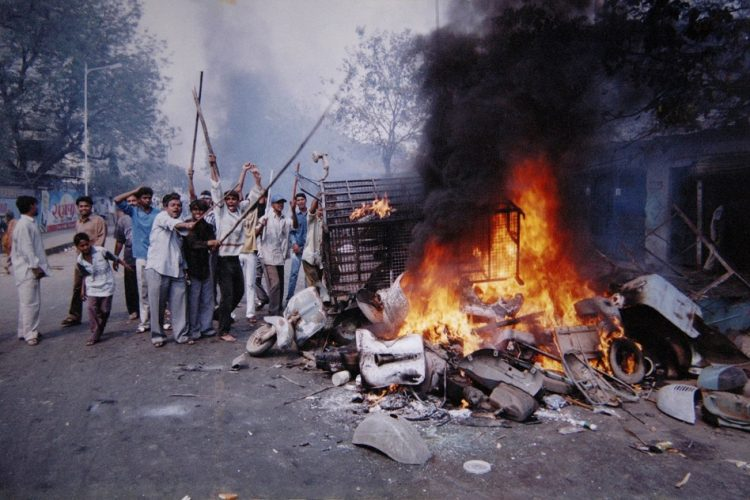
\includegraphics[width=0.8\linewidth]{img/communal-Voilence-750x500.jpg}
	\label{cv}
\end{figure}
\end{frame}

\begin{frame}
\frametitle{Communal violence}
\begin{figure}[htpb]
	\centering
	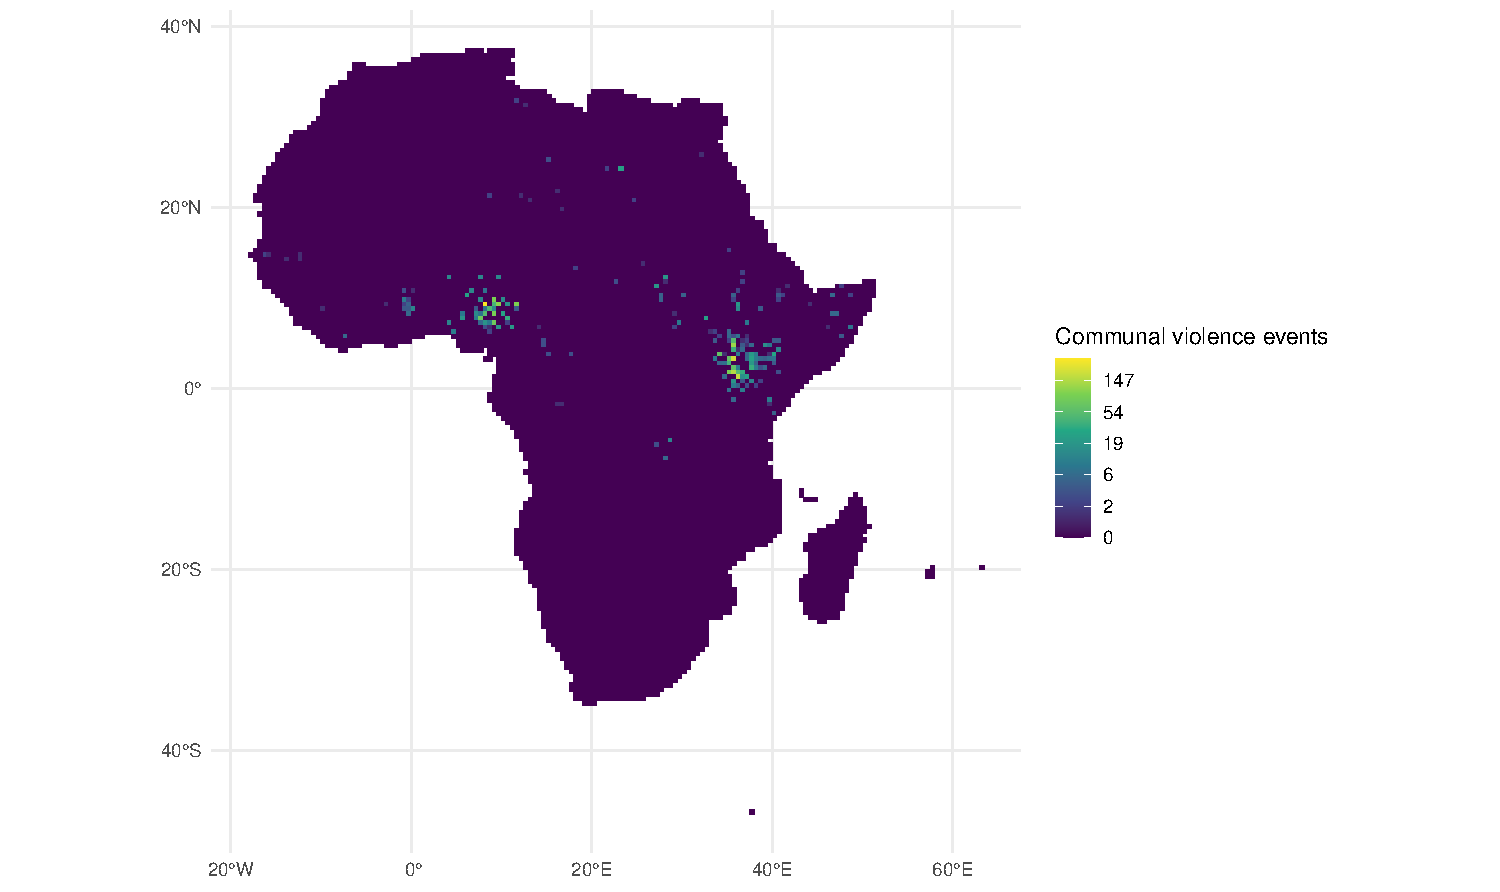
\includegraphics[width=\linewidth]{../R/Output/logOrg3.pdf}
	\caption{Communal violence (log-transformed for visualisation)}
	\label{org3}
\end{figure}
\end{frame}

\section{Peace in the absence of states}

\begin{frame}{Why are communities prone to conflict}

\begin{columns}
\column{0.5\textwidth}
\begin{itemize}
	\item[-] Information problems \pause
		% Individual reputations
		% Individual transgressions lead to collective retribution
	\item[-] Lack of credible commitments \pause
		% Lack of leaders and institutions to make commitments credible
		% by being able to punish spoilers.
		% Lack of overarching authority to prevent the stronger party
		% reneging on agreements.
	\item[-] Security dilemma 
		% The combination of the above make defensive moves look
		% threatening. Chronic uncertainty. Arms races, escalation of
		% posturing and preemptive strikes are the result.
\end{itemize}	

\column{.5\textwidth}
\begin{figure}[htpb]
	\centering
	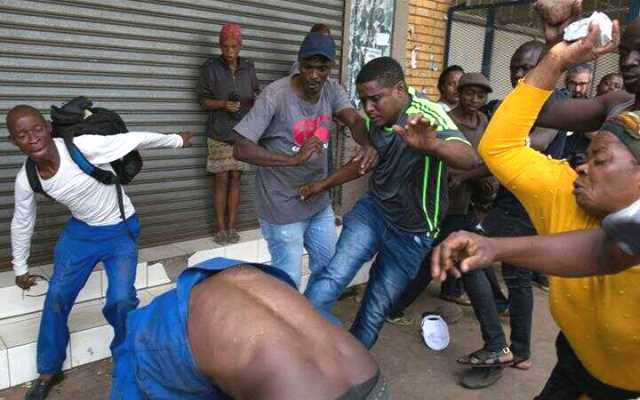
\includegraphics[width=\linewidth]{img/xenophobia.jpeg}
	\label{xeno}
\end{figure}
\end{columns}
\end{frame}

% Slide here on IGP and so on?

\section{Leviathan}

\begin{frame}{Enter Leviathan}

\begin{figure}[htpb]
	\centering
	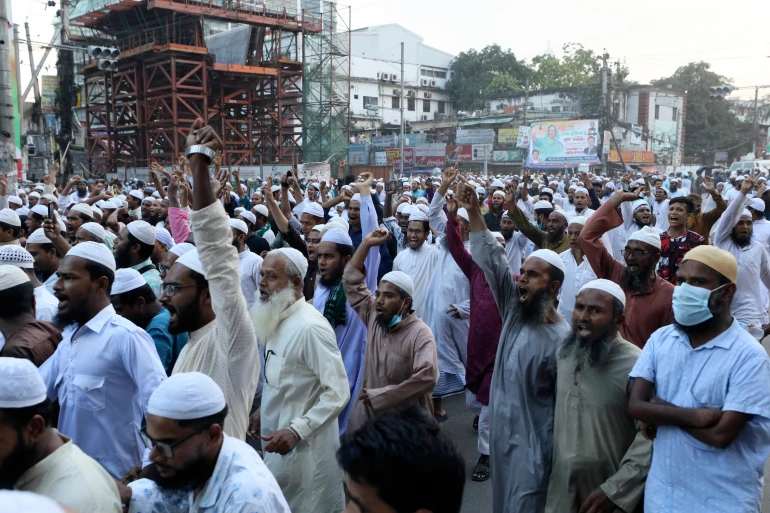
\includegraphics[width=0.8\linewidth]{img/ap.png}
	\caption{Muslims protesting against local Hindu insult to Islam...}%
	\label{ap}
\end{figure}	

\end{frame}

\begin{frame}{Enter Leviathan}

\begin{figure}[htpb]
	\centering
	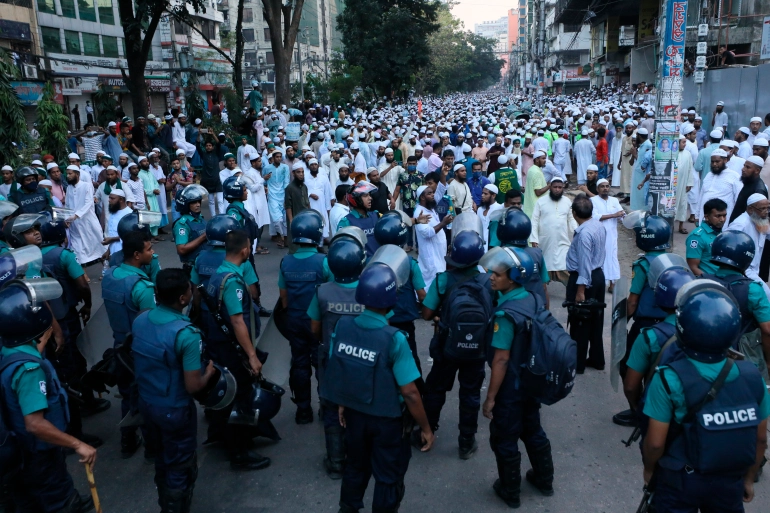
\includegraphics[width=0.8\linewidth]{img/AP.png}
	\caption{...being stopped by police}%
	\label{AP}
\end{figure}	

\end{frame}

\begin{frame}
\frametitle{Precolonial states} 

\begin{figure}[htpb]
	\centering
	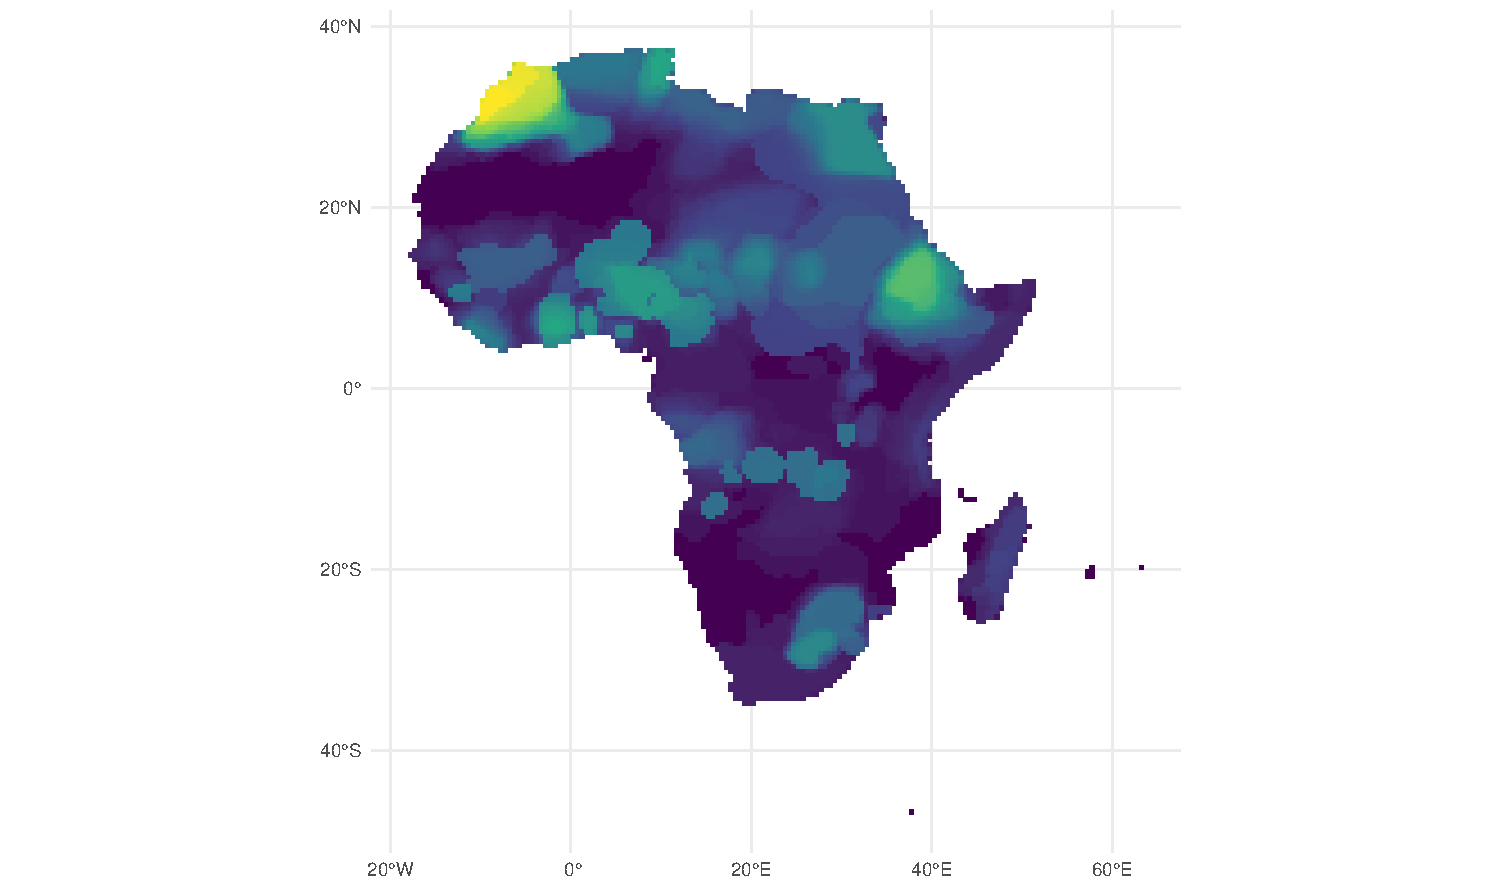
\includegraphics[width=\linewidth]{../R/Output/sqrtSpAll.pdf}
	\caption{Precolonial state presence}%
	\label{sp}
\end{figure}
\end{frame}

%\begin{frame}
%\frametitle{Precolonial states} 
%
%\begin{figure}[htpb]
%	\centering
%	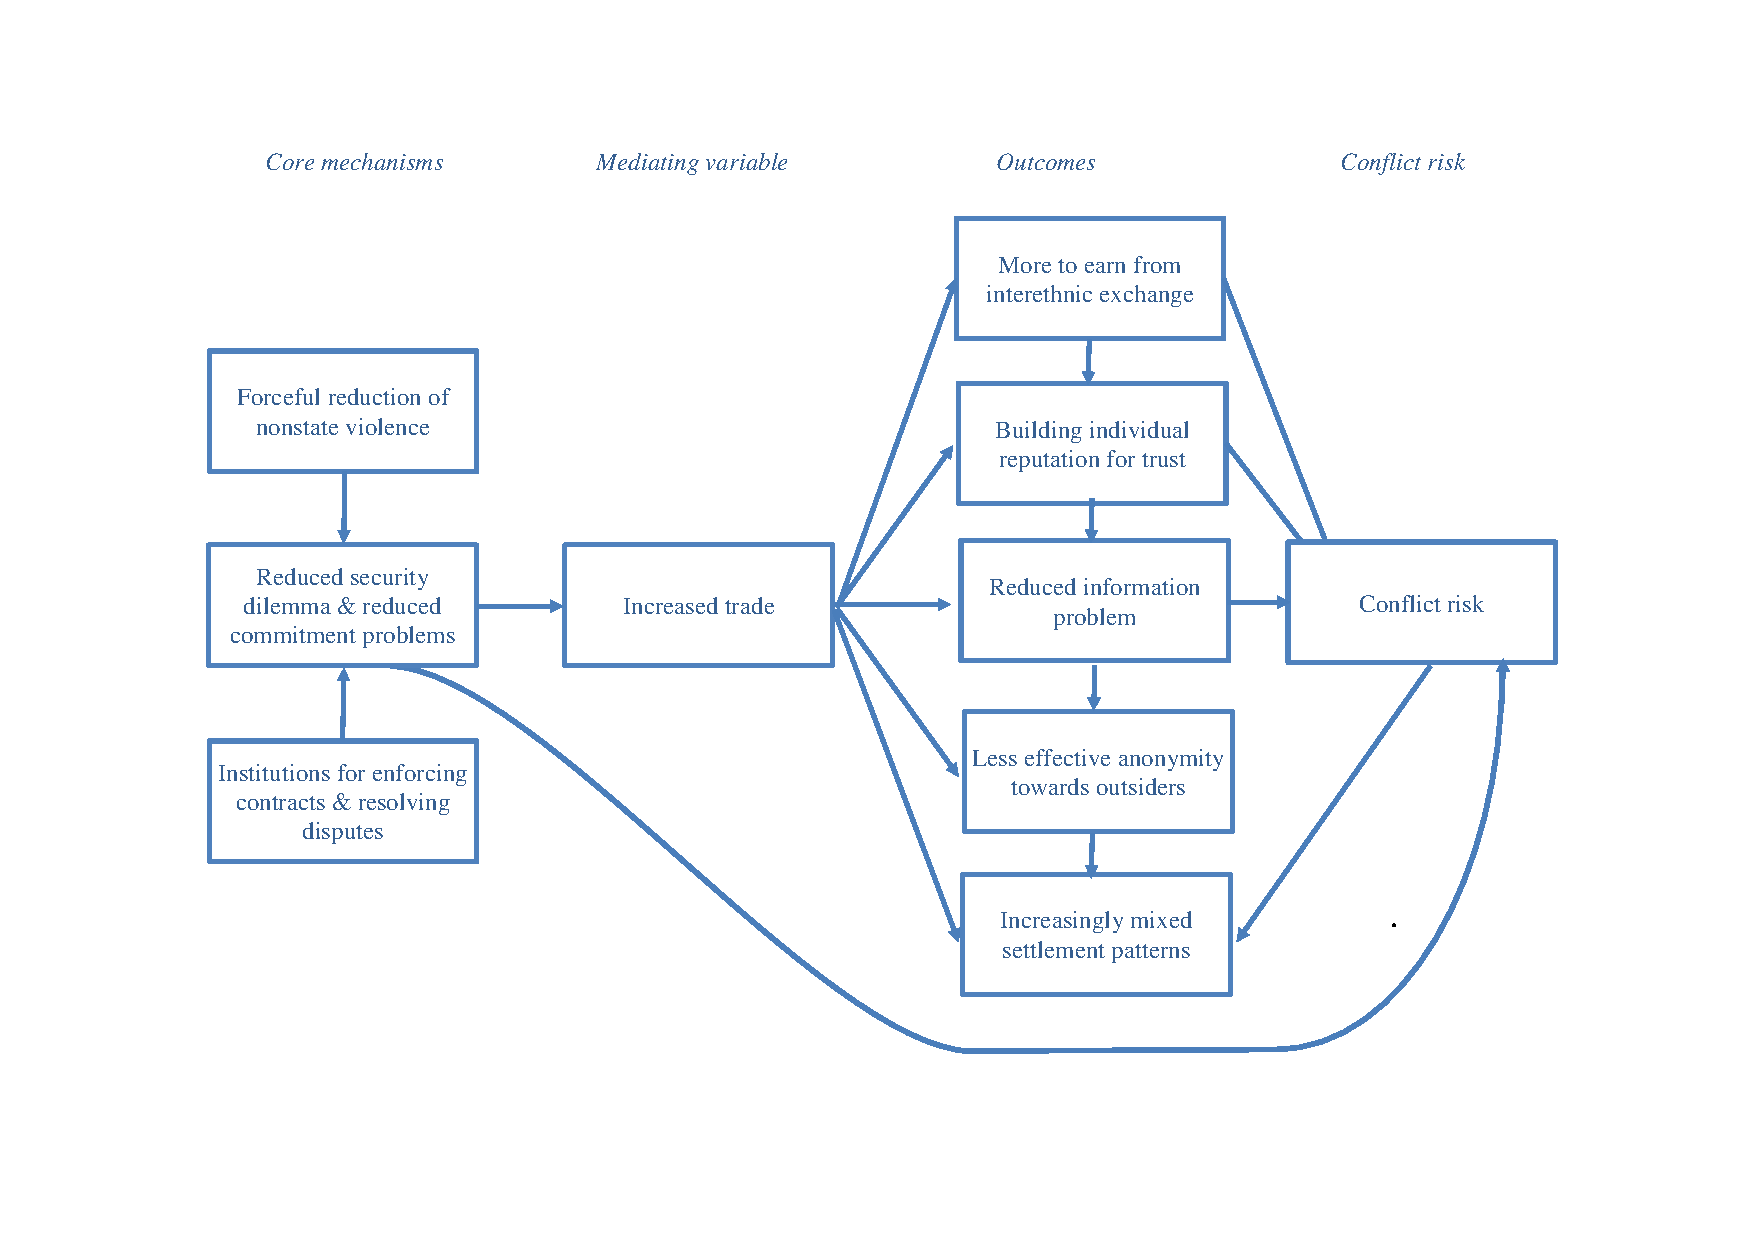
\includegraphics[width=0.9\linewidth]{img/Causal diagram.pdf}
%	\caption{Causal diagram}%
%	\label{causal}
%\end{figure}
%\end{frame}

\section{Inheritance of precolonial states}

\begin{frame}{Lasting footprints}

\begin{itemize}
	\item[-] Left over effects \pause
	\item[-] Ease of integration \pause
	\item[-] Institutions
\end{itemize}	

\end{frame}

\section{Preliminary results}

\begin{frame}{Main results}

	\begin{figure}[htpb]
		\centering
		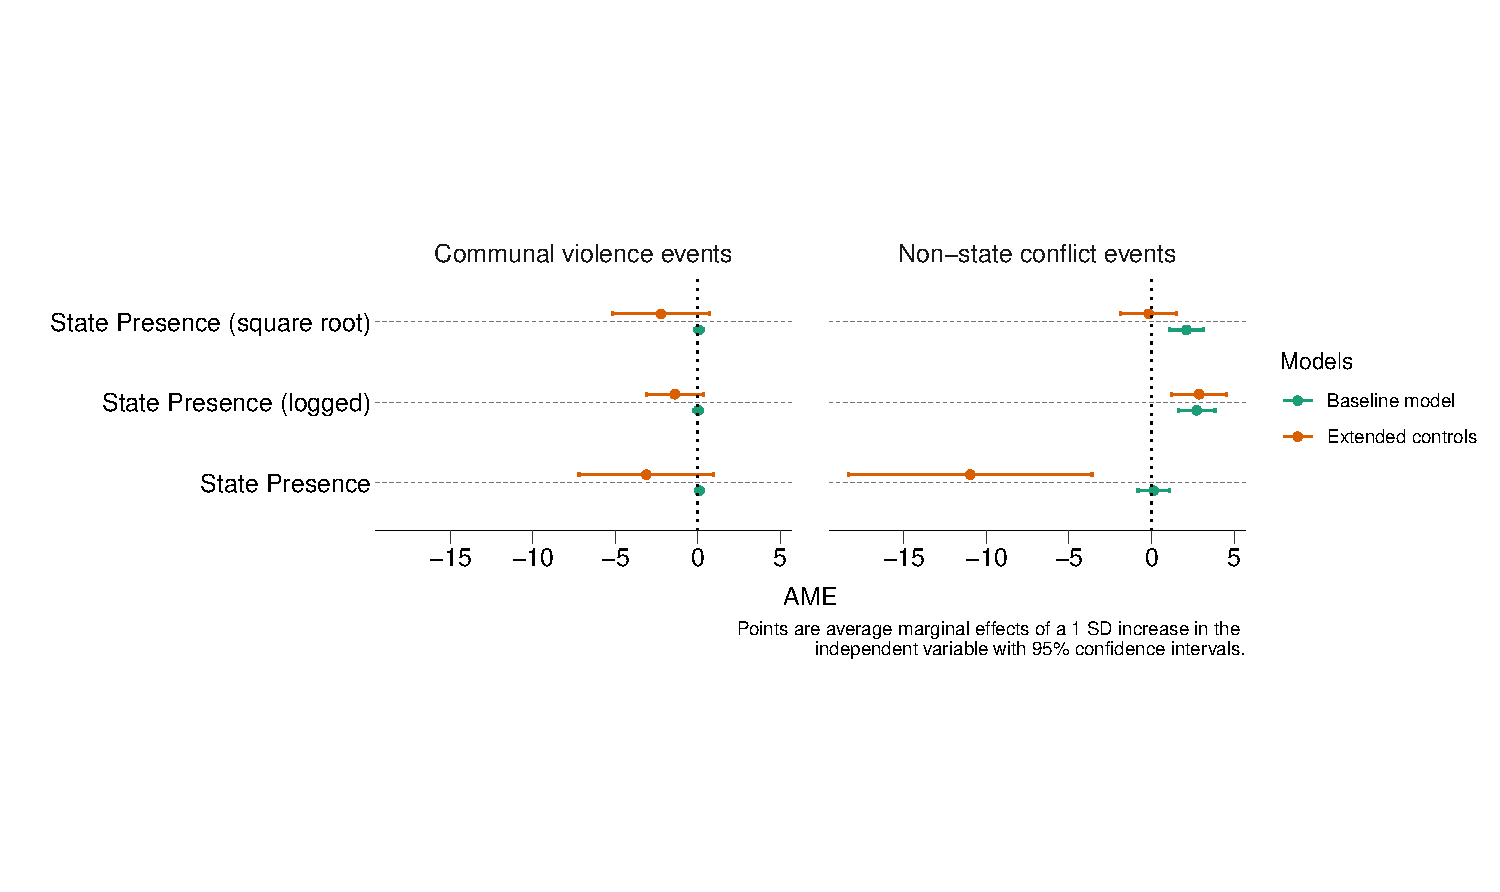
\includegraphics[width=0.8\linewidth]{../R/Output/CommunalViolenceMargins.pdf}
		\label{Margins}
	\end{figure}

	% Positive for other forms of violence, even non-state as a whole

\end{frame}

\section{What's next}

\begin{frame}{SIDE}

\begin{figure}[htpb]
	\centering
	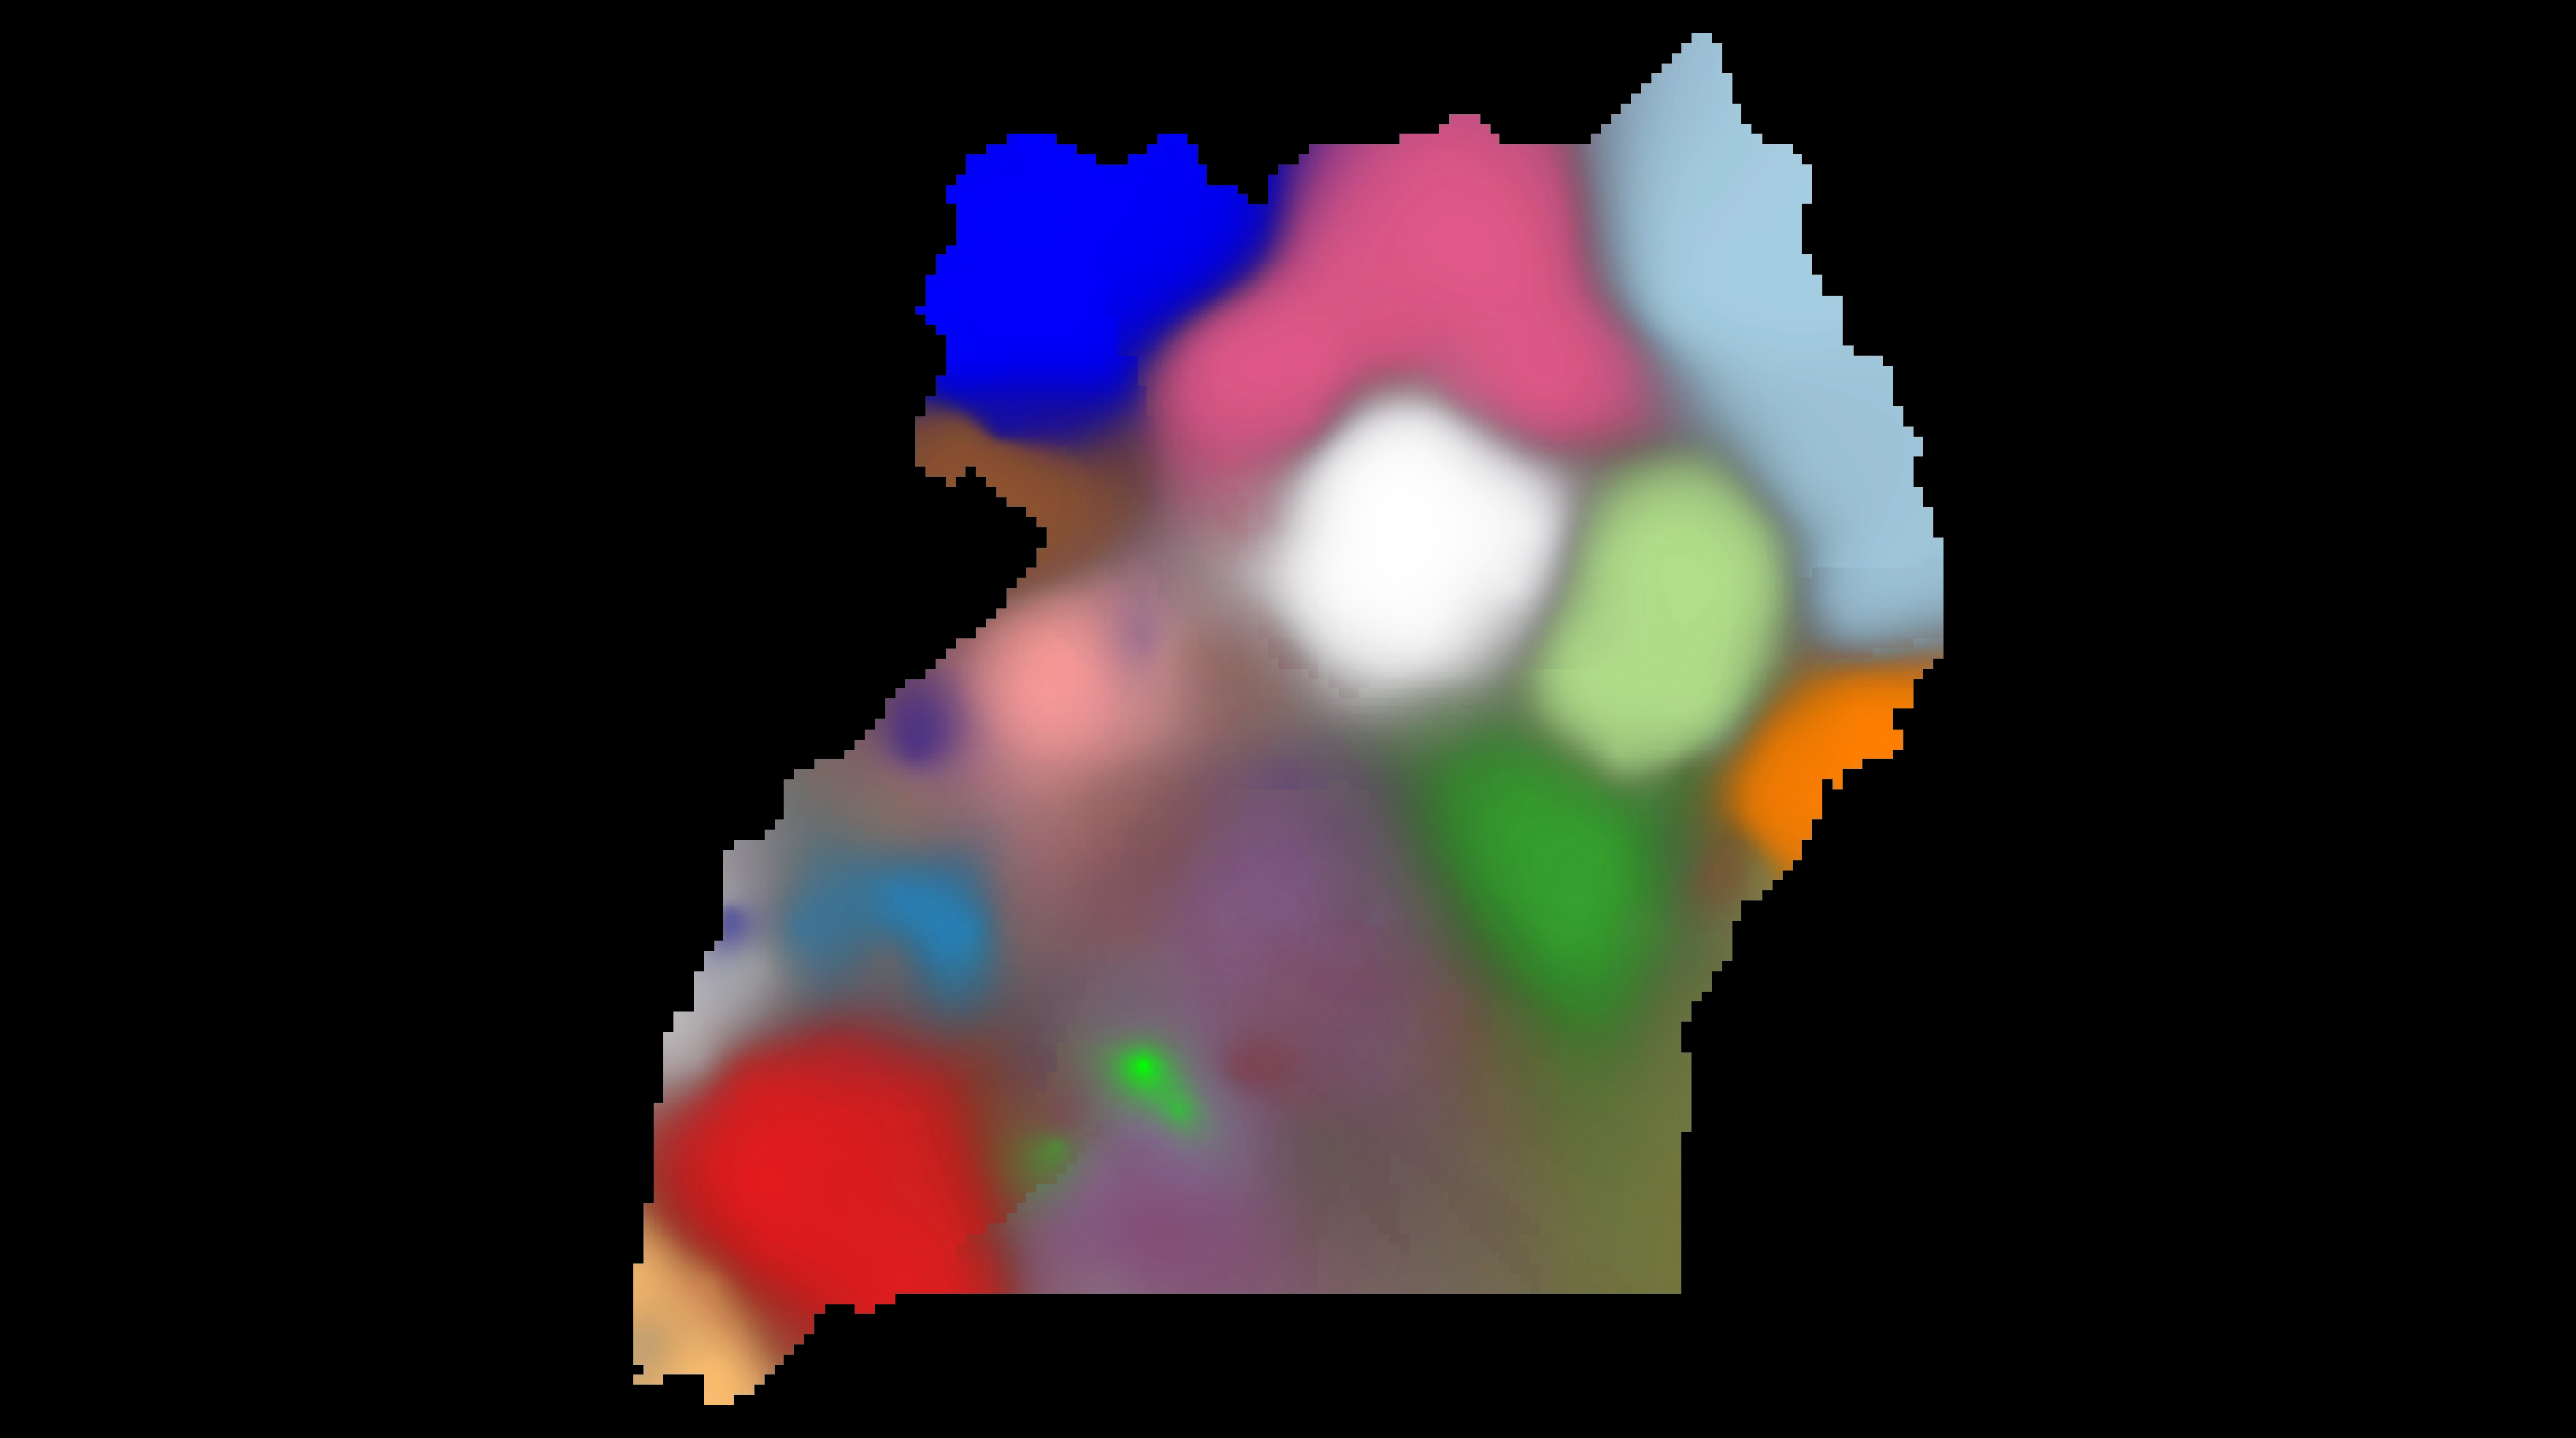
\includegraphics[width=0.8\linewidth]{img/UGA illustration1.pdf}
	\caption{Ethnic groups in Uganda}%
	\label{SIDE1}
\end{figure}	

\end{frame}

\begin{frame}{SIDE}

\begin{figure}[htpb]
	\centering
	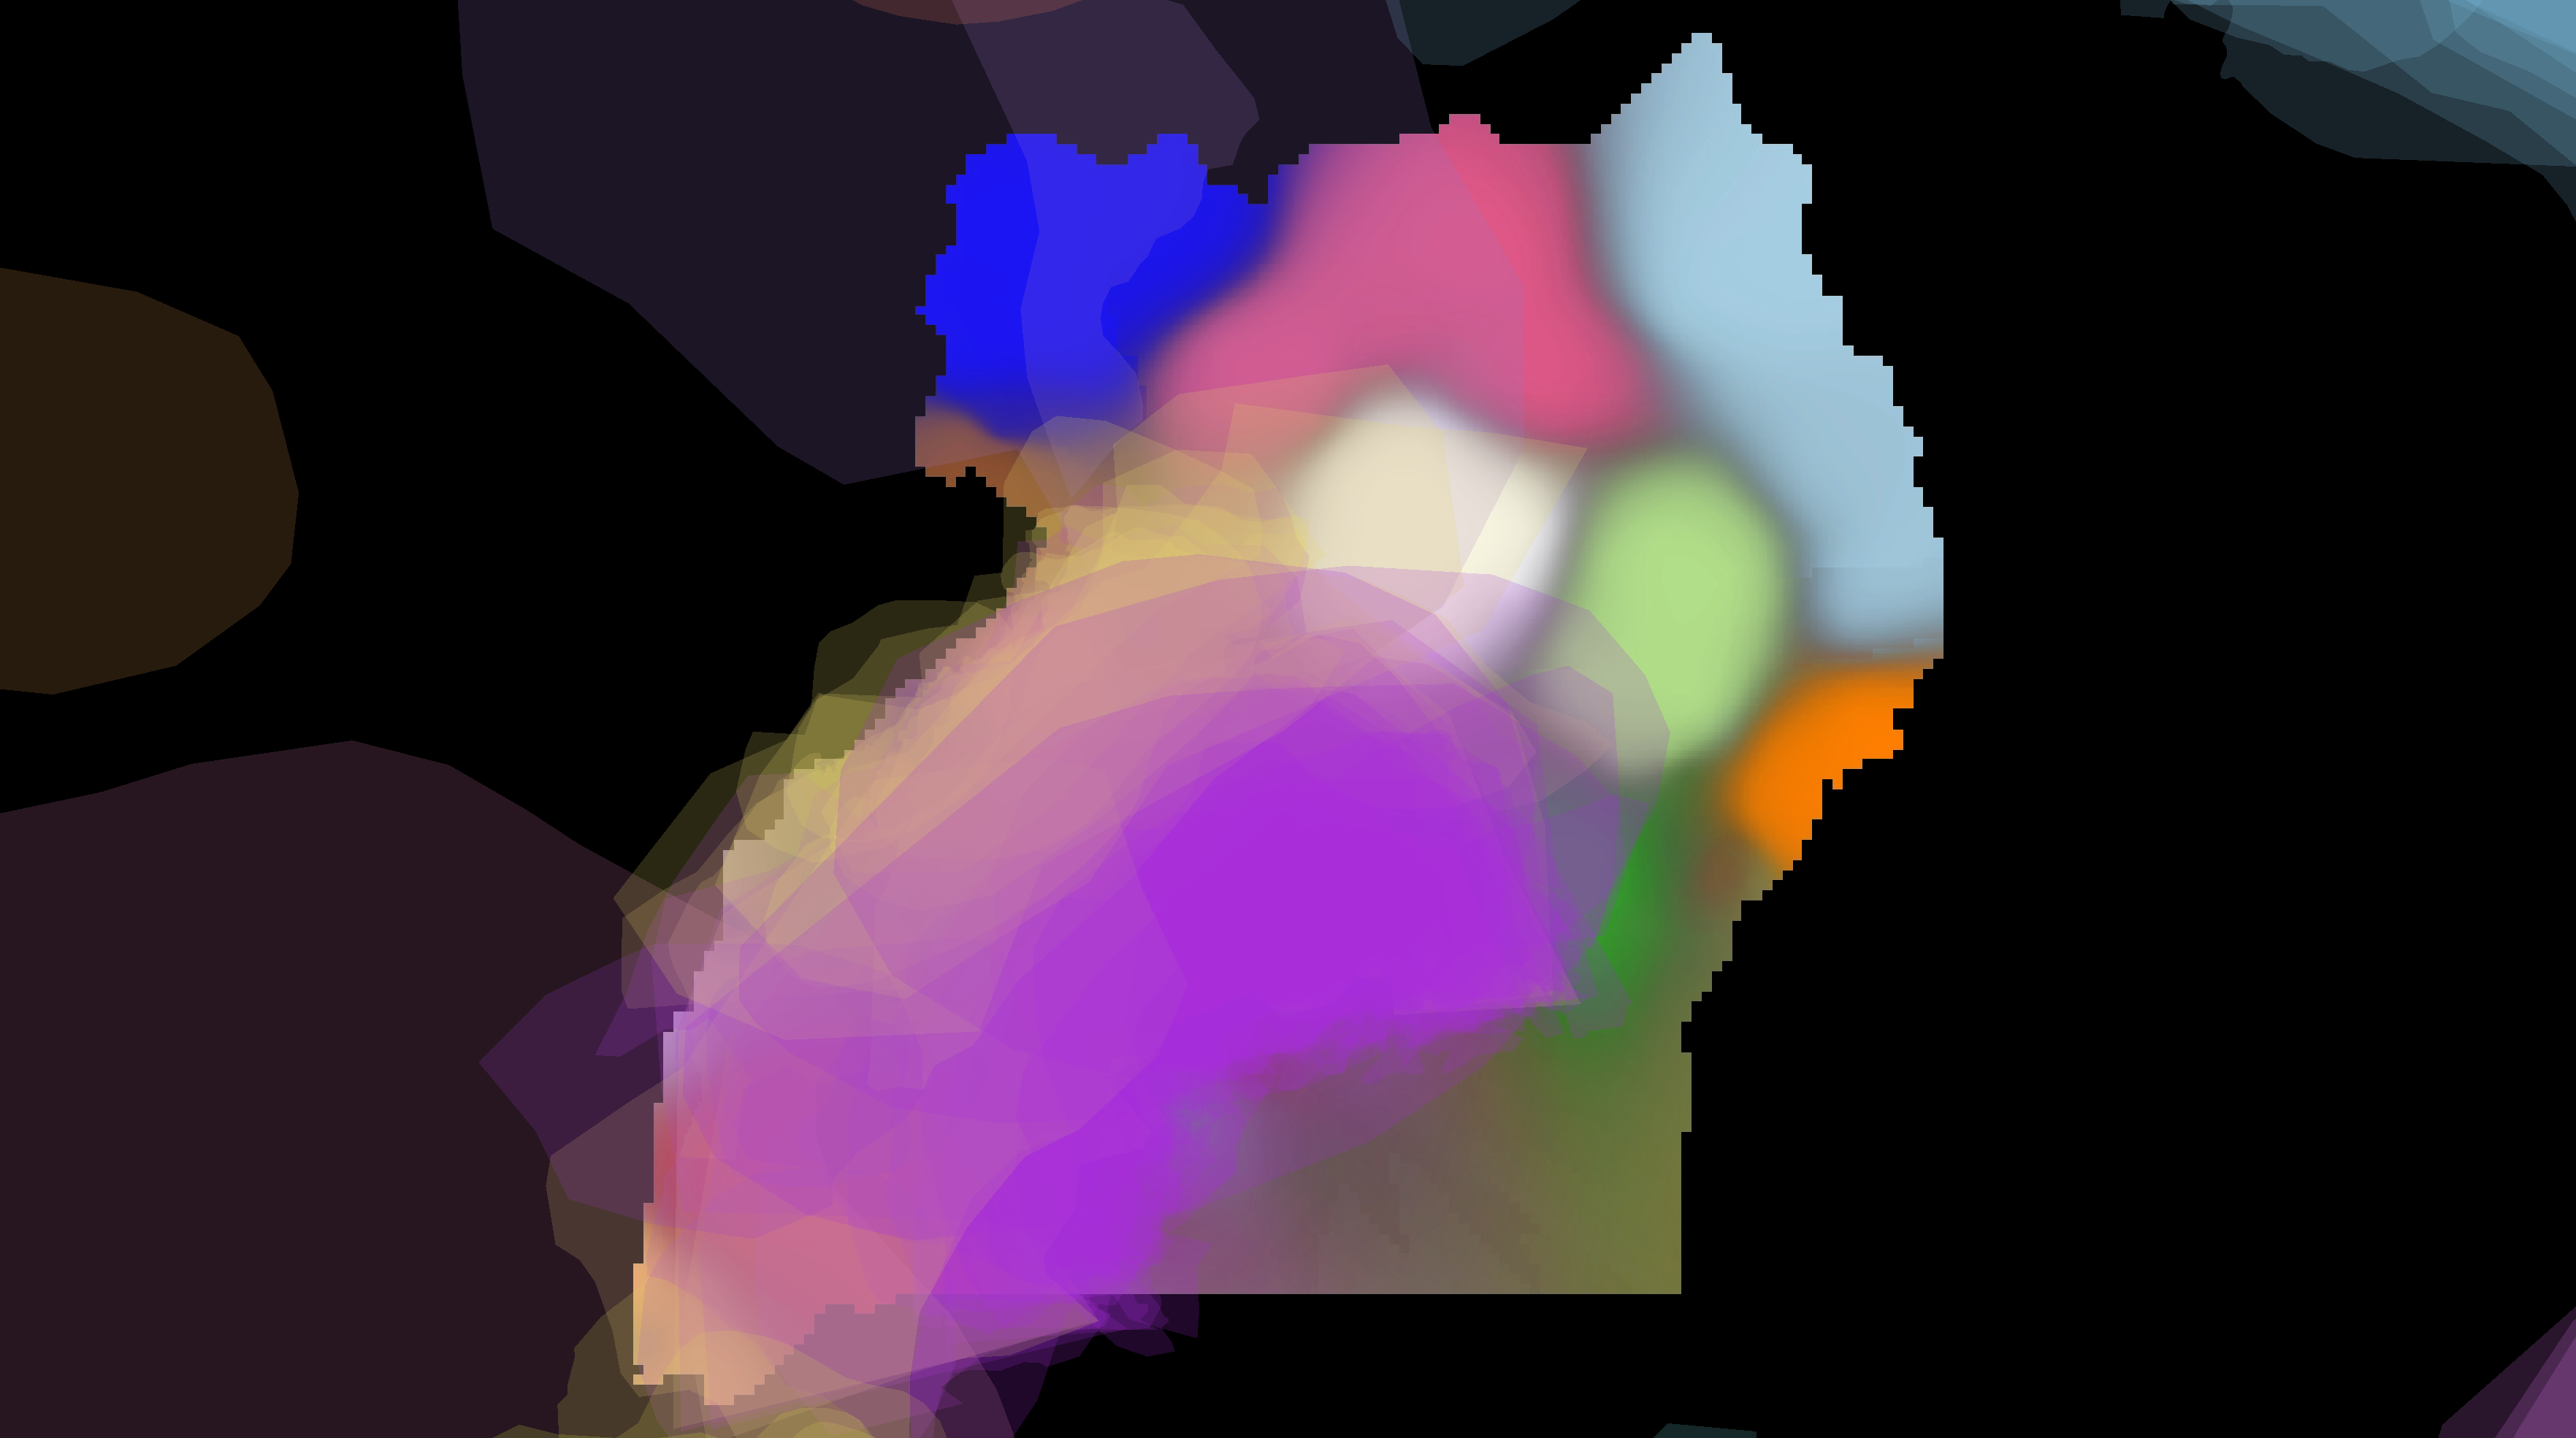
\includegraphics[width=0.8\linewidth]{img/UGA illustration2.pdf}
	\caption{Ethnic groups and precolonial states in Uganda}%
	\label{SIDE2}
\end{figure}	

\end{frame}

\begin{frame}{Afrobarometer}

	\begin{itemize}
		\item[-] Trust (general, intraethinc and interethnic) \pause
		\item[-] Identity (national or ethnic) \pause
		\item[-] Support for use of violence in politics
	\end{itemize}

\end{frame}

\end{document}	
